\chapter{模擬環境}
%\renewcommand{\baselinestretch}{10.0} %設定行距
\section{模擬模型}
 在模擬的模型上,延用了學長之前組建的實體3D列印機,並將其轉為虛擬模型後放入CoppeliaSim,進行組裝、配置並將其與GCodeInterpreter整合,用以達成使用GCode控制CoppeliaSim中的3D列印機進行模擬列印展示之功能。\\
\begin{figure}[hbt!]
\center
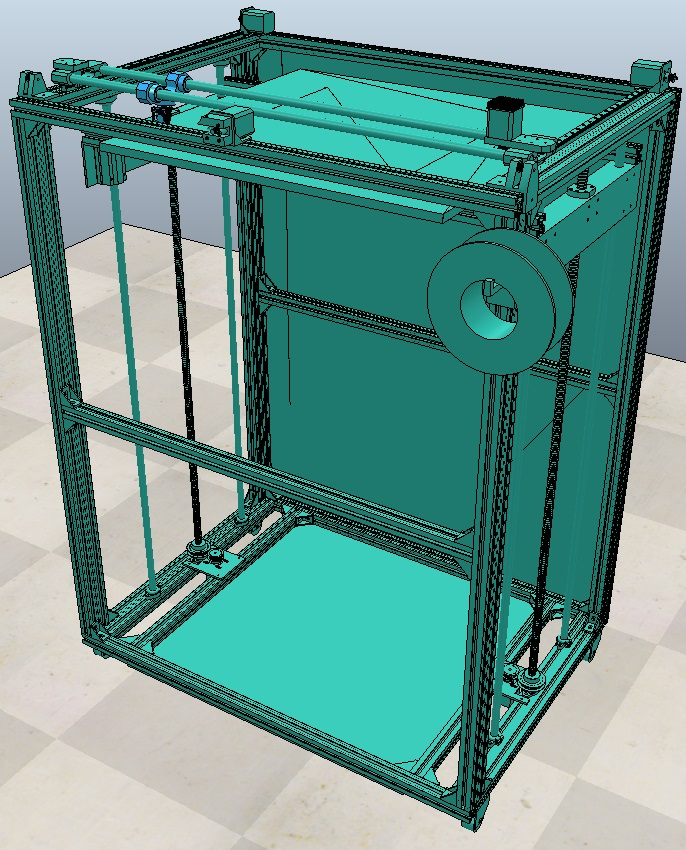
\includegraphics[width=13cm]{組合圖}
\caption{\Large 組合圖}
\label{組合圖}
\end{figure}

\newpage

\section{CoppeliaSim模擬}
 CoppeliaSim是一套具有整合開發環境的機器人模擬軟體,基於分佈式控制體系架構,可以利用寫入嵌入式腳本、插件、ROS、BlueZero節點、RemoteAPI客戶端或自定義解決方案達成模型控制之效果。\\
 \begin{figure}[hbt!]
\center

\includegraphics[width=10cm]{CoppeliaSim}
\caption{\Large CoppeliaSim Logo}
\end{figure}

並且在CoppeliaSim中,控制器可以用C / C ++、Python、Java、Lua、Matlab或Octave進行編寫。\\
\subsection{使用原因}
 本模擬之最終目標是希望可以在虛擬環境中進行3D列印的結果展示,通過虛擬環境中的模擬後,在每次修改零件並更新Gcode後可以直接展示列印的狀況,且在虛擬環境中不會有費用的支出,所以可以用於檢視所列印出之成果後,再進行圖檔修正或設計修改,除此之外CoppeliaSim的虛擬環境更接近真實環境,基於以上原因,所以此專題選擇CoppeliaSim做為模擬的環境。\\
\subsection{RemoteAPI}
 RemoteAPI(Remote Application Programming Interface)是CoppeliaSim API框架的一部分。它允許CoppeliaSim與外部應用程序之間的通訊,是跨平台並支持服務調用和雙向數據流。有兩個不同的版本/框架分別為:Remote API 和The B0-based remote API。\\
\subsection{功能列}
\begin{enumerate}
\item 以下為簡易功能說明:
\begin{figure}[hbt!]
\center
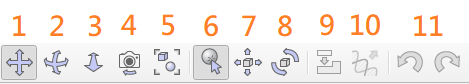
\includegraphics[width=11cm]{toolBar}
\caption{\Large CoppeliaSim 工具列}
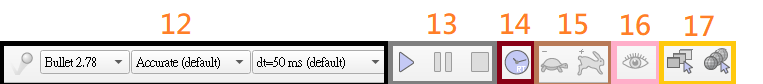
\includegraphics[width=13cm]{toolBar2}
\caption{\Large CoppeliaSim 工具列(續)}
\end{figure}
\begin{table}[hbt!]
\center
\large
\setlength{\tabcolsep}{0.75cm}{
\begin{tabular}{|c|c|c|c|}
\hline  代號 & 功能說明 & 代號 & 功能說明\\
\hline  1 &畫面平移& 10 &複製所有設定\\
\hline  2 &畫面旋轉& 11 &回復/取消回復\\
\hline  3 &畫面縮放&12&模擬設定\\
\hline  4 &畫面視角&13&開始/暫停/停止 模擬\\
\hline  5 &畫面縮放至適當大小&14&即時模擬切換\\
\hline  6 &選取物件&15&模擬速度控制\\
\hline  7 &移動物件&16&線程渲染/視覺化\\
\hline  8 &旋轉物件&17&場景/頁面 選擇\\
\hline  9 &加入/移出 樹狀結構&&\\
\hline
\end{tabular}}
\caption{\Large 功能說明}
\end{table}
\newpage
%\item 模擬執行\\%
\end{enumerate}

\newpage 